\documentclass[10pt]{report}
\usepackage{/Users/bradenhoagland/latex/math}

\lhead{Braden Hoagland}
\chead{HW 8}
\rhead{}

\renewcommand{\theenumi}{\alph{enumi}}

\begin{document}
%\tableofcontents

{\color{blue}Problems Completed: All.}

\begin{exer}[\S 22, \#2]
\begin{enumerate}
	\item $p:X\to Y$ continuous. If there is a continuous $f:Y\to X$ such that $p \circ f = 1_{Y}$, then $p$ is a quotient map.
	\item Show that a retraction $r$ of $X$ onto $A$ is a quotient map.
\end{enumerate}
\end{exer}
{\color{blue}Collaborators: None.}
\begin{enumerate}
	\item Let $p:X\to Y$ be continuous, and suppose there is some other continuous $f:Y\to X$ such that $p\circ f=1_{Y}$.
		\begin{itemize}
			\item Let $y \in Y$ be arbitrary. Then $(p\circ f)(y) = y$, so $p(f(y))=y$, so $p$ is surjective.
			\item Suppose $U$ is open in $Y$, then since $p$ is continuous $p^{-1}(U)$ is open in $X$. Conversely, suppose $p^{-1}(U)$ is open in $X$, then
				\[
					f^{-1}(p^{-1}(U)) = (p\circ f)^{-1}(U) = 1_{Y}^{-1}(U) = U.
				\] Since $f$ is continuous, this means $U$ is open.
		\end{itemize}
		Thus $p$ is a quotient map.
	\item Suppose $r:X\to A$ is a retraction onto $A$, then it is continuous and fixes $A$. We can define $\iota:A\to X$ to be the usual inclusion map, which we know to be continuous. Then $r \circ \iota = 1_{A}$, so by part (a), $r$ is a quotient map.
\end{enumerate}

\pagebreak
\begin{exer}[\S 22, \#3]
$A \subset \mathbb{R}^2$ is all points for which either $x \geq 0$ or $y=0$. Let $q = \pi_{1}|A$. Show that $q$ is a quotient map that is neither open nor closed.
\end{exer}
{\color{blue}Collaborators: Saloni.}
\textbf{$q$ is a quotient map:} Define a continuous map $f:\mathbb{R}\to A$ by $f(x)=(x,0)$, then $q\circ f = 1_\mathbb{R}$, so by Exercise 1 part a, $q$ is a quotient map onto $\mathbb{R}$.

\textbf{$q$ is not open:} Let $U$ be the open rectangle $\left\{ (x,y) \;\; -1<x<1, 1<y<2 \right\}$ in $\mathbb{R}^2$. Then $U \cap A = \left\{ (x,y) \;|\; 0\leq x < 1, 1 < y < 2 \right\}$ is open in $A$. Its projection onto $\mathbb{R}$ is the interval $[0,1)$, which is not open in $\mathbb{R}$, so $q$ is not an open map.

\begin{figure}[H]
	\centering
	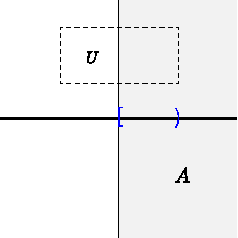
\includegraphics[scale=1]{fig/not-open.pdf}
\end{figure}

\textbf{$q$ is not closed:} As proved in Homework 6 Exercise 4, the graph of a continuous function whose codomain is Hausdorff must be closed. Thus the graph $G_f$ of $f(x) = 1/x$ for $x>0$ is closed in $A$. But $q(G_{f})=(0,\infty)$ is not closed in $\mathbb{R}$, so $q$ is not a closed map.

\begin{figure}[H]
	\centering
	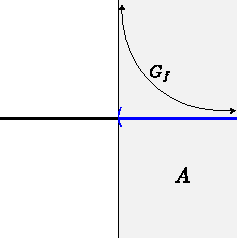
\includegraphics[scale=1]{fig/not-closed.pdf}
\end{figure}

\pagebreak
\begin{exer}[\S 22, \#4]
\begin{enumerate}
	\item Let $X = \mathbb{R}^2$. Define $(x_0,y_0) \sim (x_1,y_1) \iff x_0+y_0^2=x_1+y_1^2$. What is $X^{*}$ homeomorphic to?
	\item Repeat (a) for $(x_0,y_0) \sim (x_1,y_1) \iff x_0^2+y_1^2=x_1^2+y_1^2$.
\end{enumerate}
\end{exer}
{\color{blue}Collaborators: None.}
\begin{enumerate}
	\item Let $g(x,y) = x+y^2$, then $g$ is a continuous map that induces $\sim$, so $g(X) \cong X^*$ if and only if $g$ is a quotient map. Define a continuous map $f:\mathbb{R}\to X$ by $f(x)=(x,0)$, then $g \circ f = 1_{\mathbb{R}}$, so by Exercise 1 part (a), $g$ is a quotient map onto $\mathbb{R}$. Thus $X^{*}\cong g(X) = \mathbb{R}$.

	\item Let $g(x,y)=x^2+y^2$, then just as in part (a), $g(X) \cong X^{*}$ if and only if $g$ is a quotient map. Define a continuous map $f:\mathbb{R}_{\geq 0}\to X$ by $f(x)=(\sqrt{x} ,0)$. Then $g \circ f=1_{\mathbb{R}_{\geq 0}}$, so $g$ is a quotient map onto $\mathbb{R}_{\geq 0}$. Thus $X^{*}\cong g(X)=\mathbb{R}_{\geq 0}$.
\end{enumerate}

\pagebreak
\begin{exer}[]
	Define $(x,y,z) \sim (-x,-y,-z)$ and denote the resulting quotient space by $\mathbb{R}\mathbb{P}^2$. Consider
	\begin{align*}
		g:S^2&\to \mathbb{R}^4 \\
		(x,y,z)&\mapsto (x^2-y^2,xy,xz,yz).
	\end{align*}
	\begin{enumerate}
		\item Prove $g:S^2\to g(S^2)$ is a quotient map.
		\item Prove that $\mathbb{R}\mathbb{P}^2 \cong g(S^2)$ with the subspace topology.
	\end{enumerate}
\end{exer}
{\color{blue}Collaborators: Saloni.}
\begin{enumerate}
	\item The function $g:S^2\to g(S^2)$ is surjective because it's onto its image, and it's continuous since each of its components are continuous. Then since $S^2$ is compact (it's closed and bounded in $\mathbb{R}^n$) and $g(S^2)$ is Hausdorff (it's a subspace of $\mathbb{R}^4$, which is Hausdorff), $g$ is a closed map. Since it's closed and continuous, it is a quotient map.
	\item Now to show $\mathbb{R}\mathbb{P}^2 \cong g(S^2)$, we can show that $g$ induces the same partition of $S^2$ that $\sim$ does. Suppose $\mathbf{x} := (x,y,z) \sim (\tilde{x},\tilde{y},\tilde{z}) =: \mathbf{y}$, then we manually check that $f(\mathbf{x})=f(\mathbf{y})$.

		Conversely, given $f(\mathbf{x}) = (a,b,c,d) = f(\mathbf{y})$, we wish to find all possible values of $\mathbf{y}$. We have the system
		\[
		x^2-y^2=a, \quad xy=b, \quad xz=c, \quad yz=d.
		\] 
		In the case that $x=0$, the first equation gives $-y^2=a$, which forces both to be 0. This then makes $b=c=d=0$. Since we're on $S^2$, we know $x^2+y^2+z^2=0+0+z^2=1$, so $z = \pm 1$. Then the only possible values for $\mathbf{y}$ are $\pm(0,0,1) = \pm (x,y,z)$.

		In the case that $x \neq 0$, the second equation gives $y=b/x$, and substituting into the first and multiplying both sides by $x^2$ gives the polynomial
		\[
			(x^2)^2 - ax^2-b^2=0.
		\] By the quadratic formula, this has solutions
		\[
			x^2 = \frac{a \pm \sqrt{a^2 +4b^2}}{2} .
	\] Substituting our expressions for $a$ and $b$ from our system of equations into this expression yields
	\[
		x^2 = \frac{x^2-y^2 \pm (x^2+y^2)}{2} .
	\] If we use $-(x^2+y^2)$, then this becomes $x^2=-y^2$, which is impossible since one side is always positive and the other side is always negative. Thus $x^2$ can only satisfy
	\[
	x^2 = \frac{a + \sqrt{a^2+4b^2} }{2},
\] and similarly, $y^2 = (-a + \sqrt{a^2+4b^2} )/2$, which means that $\tilde{x}$ and $\tilde{y}$ are determined up to their sign by the first equation in our system. Then by our second equation $xy=b$, we have two possibilities: $(\tilde{x},\tilde{y}) = \pm (x,y)$.

Then by our last two equations $xz=c, yz=d$, we know that $\tilde{z}$ must match the sign of $\tilde{x}$ and $\tilde{y}$, i.e $\mathbf{x} =\pm\mathbf{y}$.

Thus $g$ induces $\sim$, so $g(S^2) \sim \mathbb{R}\mathbb{P}^2$.
\end{enumerate}

\end{document}
